\chapter{Introduction}

\section{Exciting astrophysics happen far, far away}

We live in a boring part of the Universe. This allows life and the life sciences to thrive here. However, everything that is interesting in astrophysics takes place far, far away. For example, most \gls{grbs} take place about 1 Gpc away from us. That is over three billion light years away! 

Why are \gls{grbs} interesting? Well, in short, they are Nature's most powerful accelerators and they outshine an entire galaxy when they occur, with luminosity $\sim10^{52}\,\mbox{erg/s}$. What is more, the physics behind these exotic events continue to remain mysterious for over 50 years. Figure~\ref{grb} shows a depiction of a \gls{grb}.

\begin{figure}
\centering
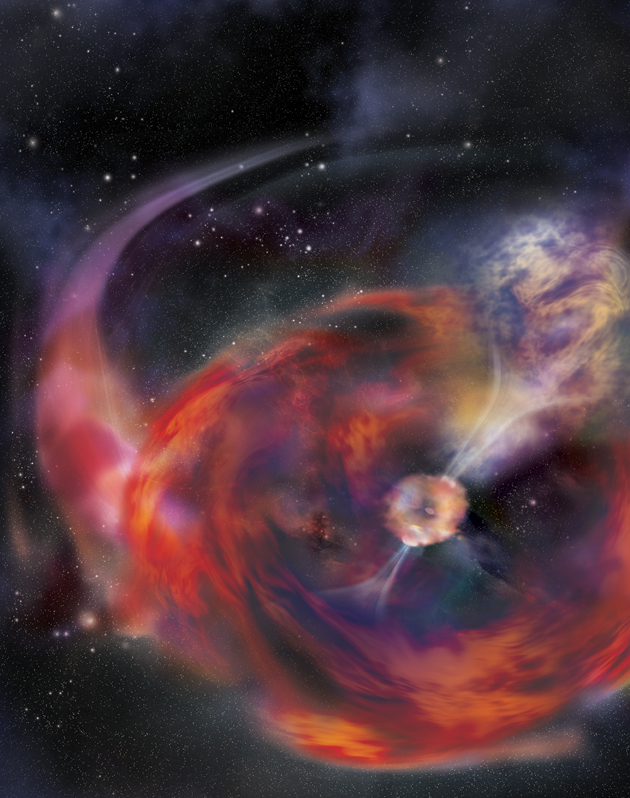
\includegraphics[width=0.5\textwidth]{figures/grb_xmas.jpg}
\caption{Depiction of a GRB. Picture Credit: NASA E/PO, Sonoma State University, Aurore Simonnet.}
\label{grb}
\end{figure}

\section{Astrophysical messengers}

Traditional astrophysical messengers are not able to completely probe physics that take place at the farthest distances and at the highest energies. Since the beginning of astronomy, we have relied on optical light to study objects in the sky. In the last few decades, we have started utilizing light of other wavelengths such as X-rays and gamma rays. However, light of energy 1~MeV and above can undergo pair production. Light of energy 13.6~eV gets absorbed by Hydrogen atoms, the most abundant element in the Universe, while light at other wavelengths gets absorbed by other atoms and molecules. Light is the astronomer's best friend, but there is an inevitable need for complementary messengers.

Fortunately, in the last century, we have opened up multiple new windows to peer into the Universe. 
About a 100 years ago, cosmic rays were discovered by Victor Hess in a balloon-based experiment. In the last several years, the IceCube neutrino observatory has discovered the first astrophysical neutrinos up to energies of a few PeV~\cite{icecube_first_pev}. Moreover, gravitational waves were discovered by the LIGO collaboration in the last few years, confirming, for example, the association of short \gls{grbs} with neutron star - neutron star mergers~\cite{ligo_short}. Figure~\ref{messengers} summarizes the astrophysical messengers we have discovered so far.

%\begin{figure}
%\centering
%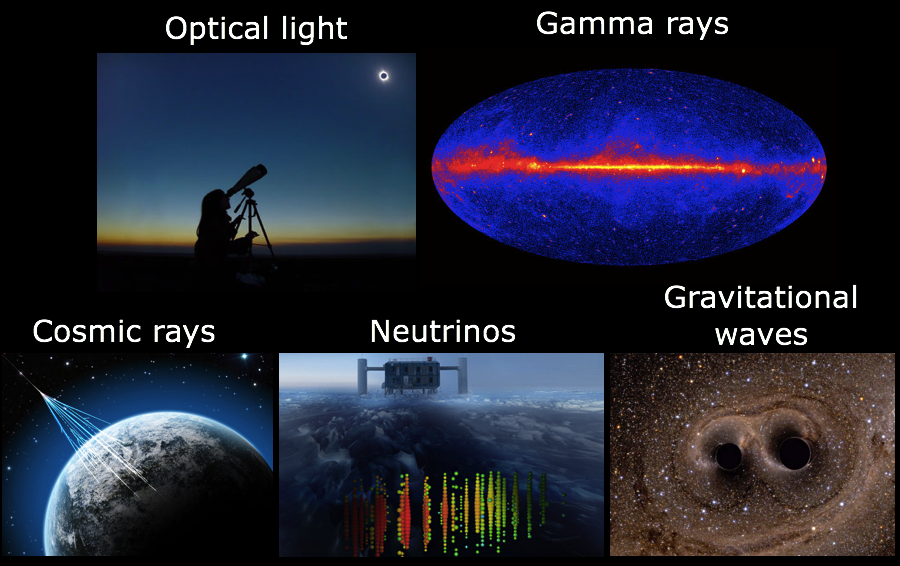
\includegraphics[width=1.0\textwidth]{figures/messengers.png}
%\caption{Astrophysical messengers. Pictures are all borrowed from Fermi, IceCube and LIGO collaborations, and the Internet.}
%\label{messengers}
%\end{figure}

\begin{figure}
\centering
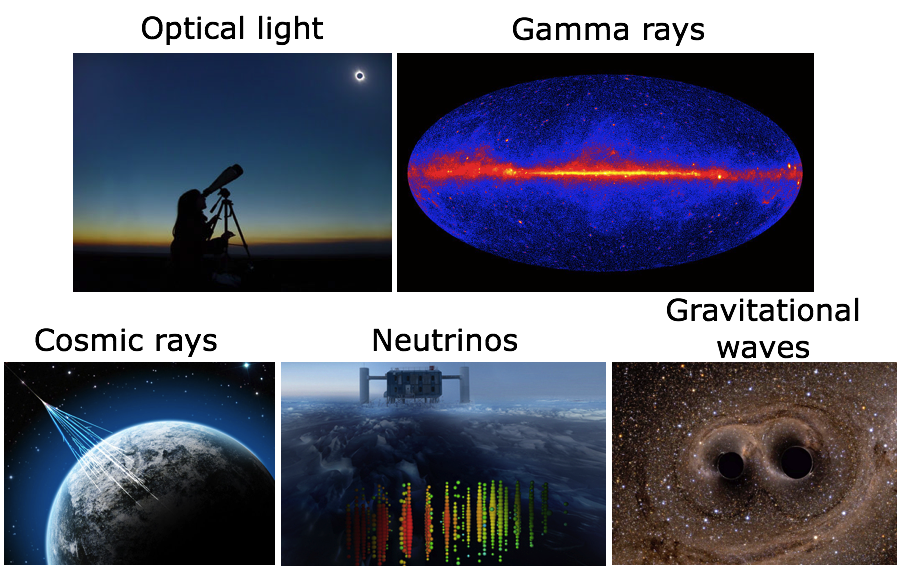
\includegraphics[width=1.0\textwidth]{figures/messengers_2.png}
\caption{Astrophysical messengers. Pictures are all borrowed from Fermi, IceCube and LIGO collaborations, and the Internet.}
\label{messengers}
\end{figure}

\section{Neutrinos as astrophysical messengers}

Neutrinos are potentially perfect candidates for carrying information about distant particle accelerators all the way to us. Due to being neutral and weakly interacting, neutrinos would remain unattenuated and point straight back to their source. In this way, they would have a definite advantage over messengers such as cosmic rays. Neutrinos are the side product of almost every nuclear reaction and can carry versatile information about particle physics taking place at cosmic distances. Their association with sources such as \gls{grbs} would confirm, for example, whether protons, in addition to electrons, get shock accelerated in the fireball model of the \gls{grb}~\cite{Waxmanreview}.

Despite a lack of observation so far, \gls{uhe} ($>10^{18}\,\mbox{eV}$) neutrinos are predicted to be produced in two ways, the more commonly referenced of which is known as the cosmogenic method. The cosmogenic method entails the interaction of cosmic rays with \gls{cmb} photons, as depicted in Figure~\ref{cosmogenic}. \gls{uhe} cosmic rays are predicted to travel only about 50 Mpc before they interact with \gls{cmb} photons, a phenomenon known as the GZK Effect. This is thought to cause the sharp drop in flux at the highest energies as seen in Figure~\ref{kneeankle}. Such an interaction can also, potentially, lead to the production of \gls{uhe} neutrinos, although no cosmogenic neutrinos have been observed so far. 

The second way of producing \gls{uhe} neutrinos is the astrophysical method, which is the one I find to be more motivating.
The astrophysical method involves the production of \gls{uhe} neutrinos in Nature's most powerful particle accelerators such as \gls{grbs}. This will be discussed in more detail in Chapter~\ref{grb}. In both the cosmogenic and astrophysical methods of producing \gls{uhe} neutrinos, a commonly referenced process of production of the same is through the interaction of a proton and a photon creating intermediate pions, as shown in Figure~\ref{uhe_process}. 

\begin{figure}
\centering
\subfloat[t]{
	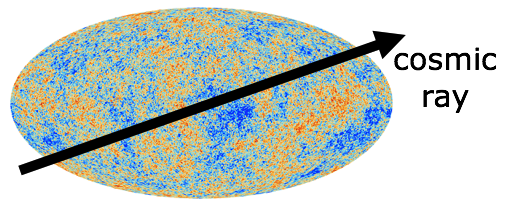
\includegraphics[width=0.8\textwidth, valign=c]	{figures/cosmogenic_2.png}
    \label{cosmogenic}
    }\quad
\subfloat[b]{
	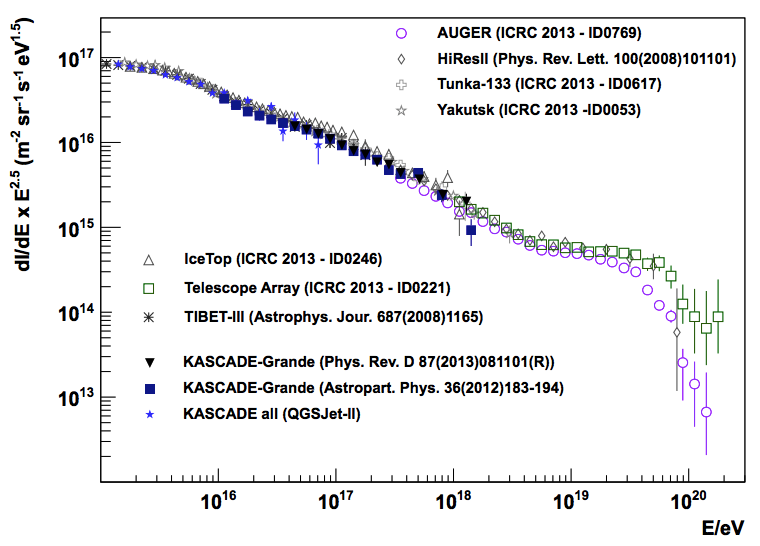
\includegraphics[width=0.8\textwidth, valign=c]{figures/kneeankle.png}
    \label{kneeankle}
    }
\caption{Top: Depiction of a cosmic ray interacting with the CMB. Thanks to the Planck telescope for the CMB picture. Bottom: Energy spectra of cosmic rays measured by different experiments. Andreas Haungs showed this plot at the 13th International Conference on Topics in Astroparticle and Underground Physics. UHE cosmic rays can only travel for about 50 Mpc before they interact with CMB photons and lose energy, therefore, we see a sharply falling spectrum at about $10^{20}\,\mbox{eV}$ energy.}
\label{cr}
\end{figure}

\begin{figure}
\centering
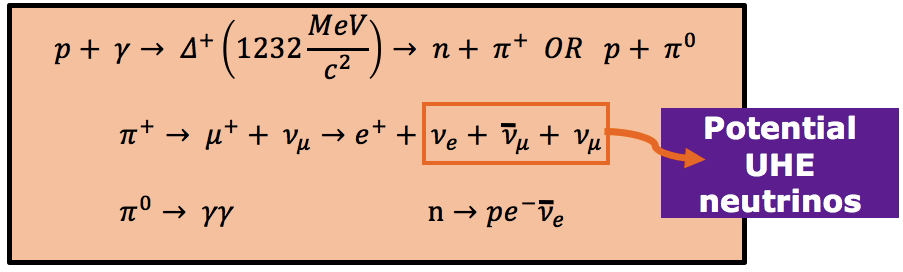
\includegraphics[width=1.0\textwidth]{figures/uhe_process.png}
\caption{A process for production of UHE neutrinos.}
\label{uhe_process}
\end{figure}

\section{Optical Cherenkov neutrino detectors}

Optical Cherenkov neutrino experiments look for high energy neutrinos in the energy regime of $10^{11} - 10^{15}\, \mathrm{eV}$. In this section, we briefly introduce two optical Cherenkov experiments, IceCube and ANTARES. Being located in complementary hemispheres of the earth, these two experiments have complementary fields of view. Where they are on the energy scale as compared to other particle physics experiments is shown in Figure~\ref{anita_energy}.

IceCube is the optical Cherenkov detector in the southern hemisphere. The observatory is located in the South Pole. The completed IceCube observatory is composed of $5160$ digital optical modules (DOMs), each containing a $10-$inch photomultiplier tube, with $60$ DOMs placed at depths between $1450$ and $2450 \, \mathrm{m}$ on each of $86$ vertical strings. The total instrumented volume of IceCube is $1 \, \mathrm{km^3}$. 

ANTARES is the optical Cherenkov detector in the northern hemisphere. It is located in the Mediterranean Sea. 
Located at a depth of $2.4 \, \mathrm{km}$, it consists of $12$ vertical strings, separated from each other by a typical distance of $70 \, \mathrm{m}$. Each string is anchored to the seabed and held upright by a buoy at the top. Over a length of $350 \, \mathrm{m}$, it is equipped with $25$ triplets of photo-multiplier tubes (PMTs), building a 3-dimensional array of $885$ PMTs in total. The instrumented volume of ANTARES is $\sim  0.02 \, \mathrm{km^3}$. 

IceCube and ANTARES are both optimized for the detection of muons from charged current interactions of high energy astrophysical neutrinos. IceCube uses the Antarctic ice as a target medium for high energy neutrinos to interact in. ANTARES uses sea-water instead. They both look for optical Cherenkov signatures of high energy neutrino interactions. ANTARES is sensitive to neutrinos of energy 10 GeV - 100 TeV. IceCube was built to detect neutrinos of energy 100 GeV and higher. However, as shown in \cite{IClow}, IceCube can also detect neutrinos of energy of order MeV. 


\begin{figure}
\centering
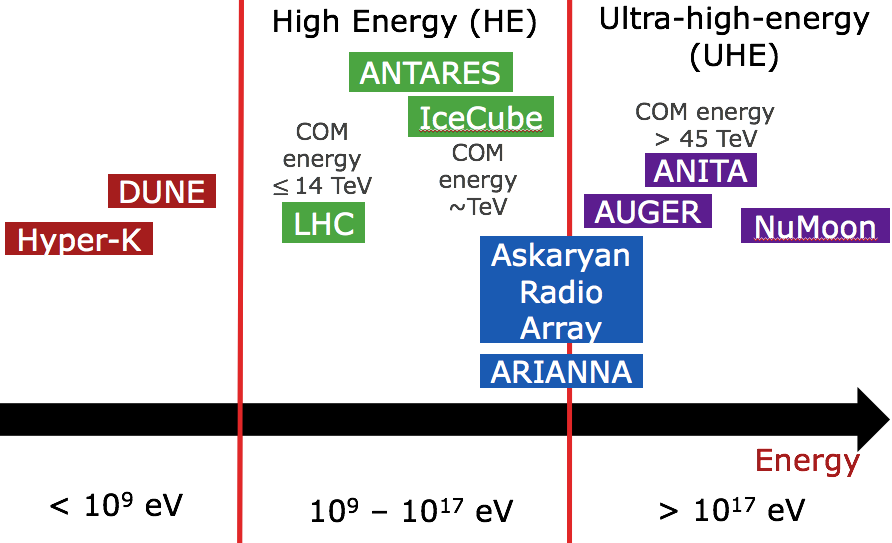
\includegraphics[width=0.9\textwidth]{figures/anita_where_energy.png}
\caption{The ANITA experiment looks for particles, specifically, neutrinos of energies that are to close to the extreme right of the energy scale.}
\label{anita_energy}
\end{figure}


\section{Radio Cherenkov neutrino detectors}

Radio Cherenkov neutrino experiments look for \gls{uhe} neutrinos in the energy regime of $> 10^{16}\,\mathrm{eV}$. The main challenge for detection by these experiments and a potential solution for detection are presented below. We also introduce two complementary radio Cherenkov experiments, \gls{anita} and \gls{ara} in this section. Where they are on the energy scale as compared to other particle physics experiments is shown in Figure~\ref{anita_energy}.

\subsection{Challenge of detecting ultra-high-energy neutrinos}

In this era of rapid growth in multi-messenger astronomy, \gls{uhe} neutrinos remain undiscovered. One of the major challenges is that observation of these rare particles requires a huge detection volume. The interaction length of an EeV neutrino and a nucleus is about 300 km. Less than 0.01 \gls{uhe} neutrinos are predicted to hit the earth per cubic kilometer per year, implying that to be sensitive to the \gls{uhe} neutrino flux we need a detection volume much greater than a 100 cubic kilometers. Such a huge detection volume would be too expensive to instrument using optical Cherenkov detectors as optical light is attenuated over order tens of meters.

\subsection{Askaryan Effect}

A proposal by~\cite{askaryan}, known as the Askaryan Effect, stating that \gls{uhe} neutrinos could be observed through their interaction in a dielectric medium, comes to the rescue. The principle is that a relativistic, \gls{uhe} neutrino would interact with a nucleus in a dielectric to produce a particle shower traveling in the medium at a speed greater than the speed of light in the medium. The particle shower would mainly consist of photons, electrons and positrons. As it travels through the dielectric, the particle shower develops about a 20\% negative charge. This happens primarily due to Compton scattering of electrons in the medium (so electrons leaving the medium and joining the shower) and secondarily due to annihilation of positrons in the shower with electrons in the medium (so positrons leaving the shower).   
As this charged particle shower travels through the medium at a speed greater than the speed of light in the medium, Cherenkov radiation is produced. If this Cherenkov radiation is observed at wavelengths larger than the shower's transverse dimension of about 10 cm, then it would be seen as coherent waves in radio frequencies. 

\begin{figure}
\centering
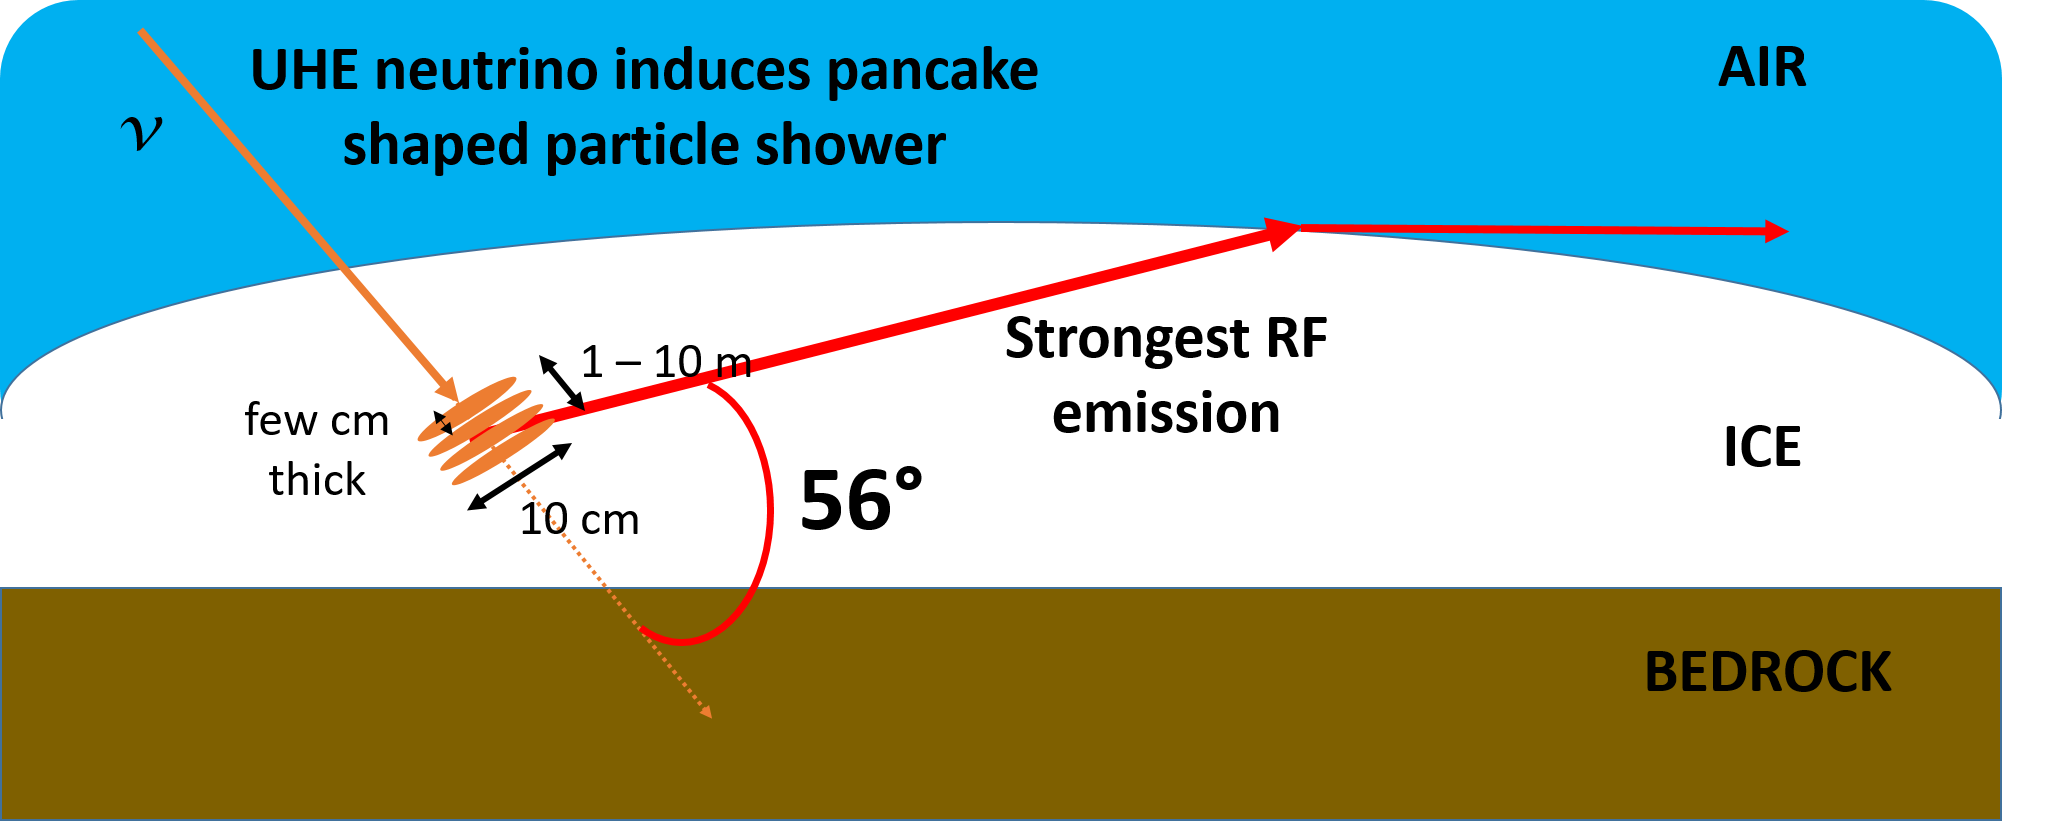
\includegraphics[width=1.0\textwidth]{figures/askaryan_in_ice.png}
\caption{A UHE neutrino could start a pancake-shaped particle shower in the ice.
Cherenkov radiation due to this particle shower would be coherent at wavelengths 
greater than the shower size of $\sim~10\,\mbox{cm}$, which correspond to radio waves.}
\label{askaryan}
\end{figure}

%ANITA and ARA use radio techniques to look for high energy neutrinos on the higher end of the energy spectrum as shown in Figure~\ref{anita_energy}. ARA covers the energy range $10^{16} - 10^{19}\, \mathrm{eV}$ which includes part of the UHE region and ANITA covers the UHE region from $10^{18}\, \mathrm{eV}$ and above. Below we provide a brief overview of these different experiments and how they complement one another.

\subsection{ANITA}

\gls{anita} is an experiment dedicated to discovering \gls{uhe} neutrinos via the Askaryan Effect utilizing the Antarctic ice as the necessary dielectric target medium for neutrino interaction. Where \gls{anita}'s sensitivity lies in the energy scale as compared to other experiments in particle physics and particle astrophysics is presented in Figure~\ref{anita_energy}. A cartoon of an \gls{uhe} neutrino coming in to the ice and starting a particle shower that leads to Cherenkov radiation emitted coherently at an angle of about $56^{\circ}$ is shown in Figure~\ref{askaryan}. \gls{anita} looks for radio Cherenkov signals with an array of radio antennas. The \gls{anita} detector is hung from a Helium-filled balloon and launched from near McMurdo Station, Antarctica, during the Austral Summer. After it is launched, \gls{anita} floats up to an altitude of about 40 km and utilizes the polar vortex to fly in roughly circular orbits over the continent of Antarctica. At its float altitude, the balloon, upon gradual inflation, is bigger than the Ohio Stadium. There have been four flights of \gls{anita} so far. These are summarized in Figure~\ref{flights_summary}.

\begin{figure}
\centering
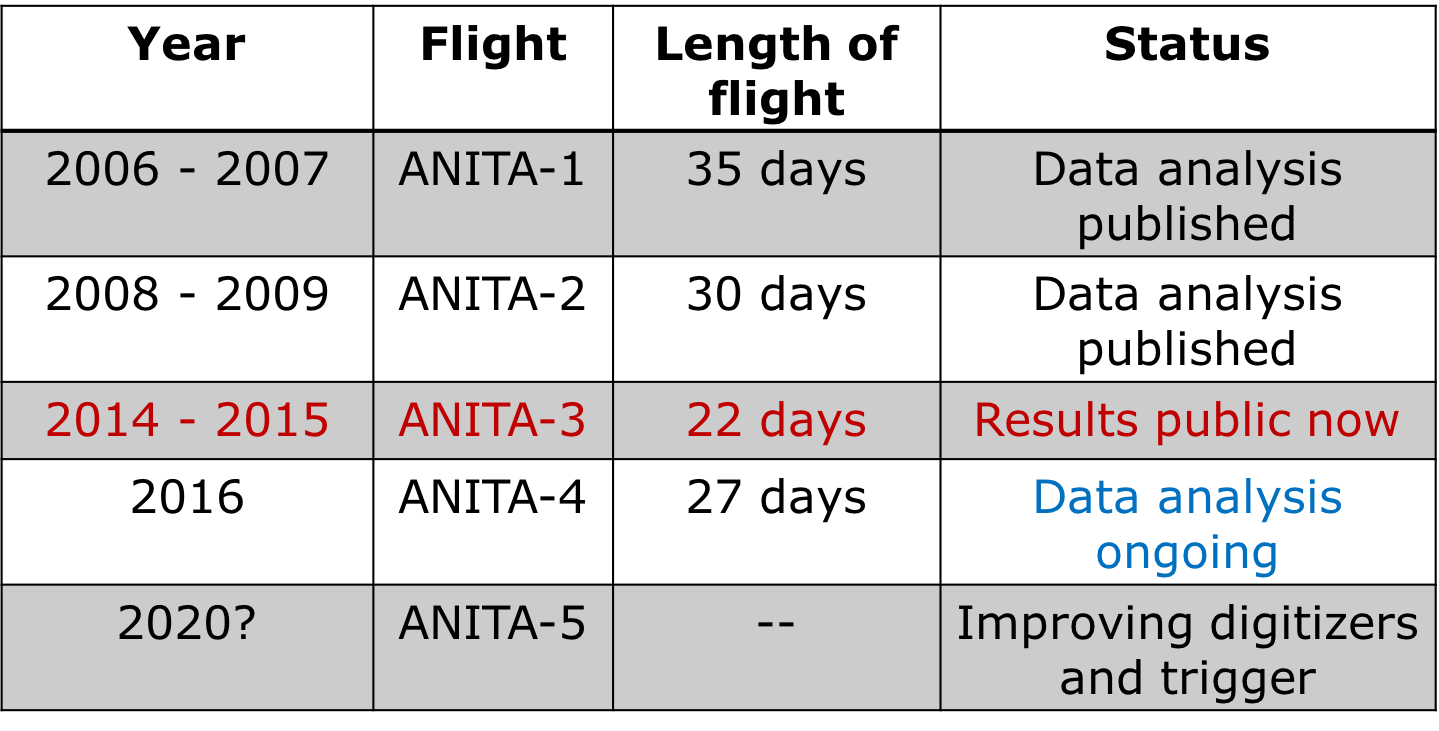
\includegraphics[width=1.0\textwidth]{figures/flights_table.png}
\caption{Summary of ANITA flights.}
\label{flights_summary}
\end{figure}

During its flight, at any given time, \gls{anita} can scan about a {\bf million} cubic kilometers of ice. This makes \gls{anita} the neutrino detector with the largest instantaneous detection volume. The use of the radio Cherenkov technique goes hand in hand with covering a detection volume that is orders of magnitude larger than what is possible with optical Cherenkov techniques such as in IceCube (1 cubic km detection volume). Radio waves have attenuation lengths of order 1 km while optical light attenuates over order tens of meter. For \gls{anita}, radio waves from neutrino cascades are produced in the ice, but then have to travel 40 km through air before they can reach the detector. Therefore, \gls{anita} is sensitive only above about an EeV neutrino energy so it is looking for the rarest neutrinos. A cartoon of radio waves from a particle shower caused by an \gls{uhe} neutrino in the ice reaching the \gls{anita} detector is shown in Figure~\ref{anita_cartoon}.

\begin{figure}
\centering
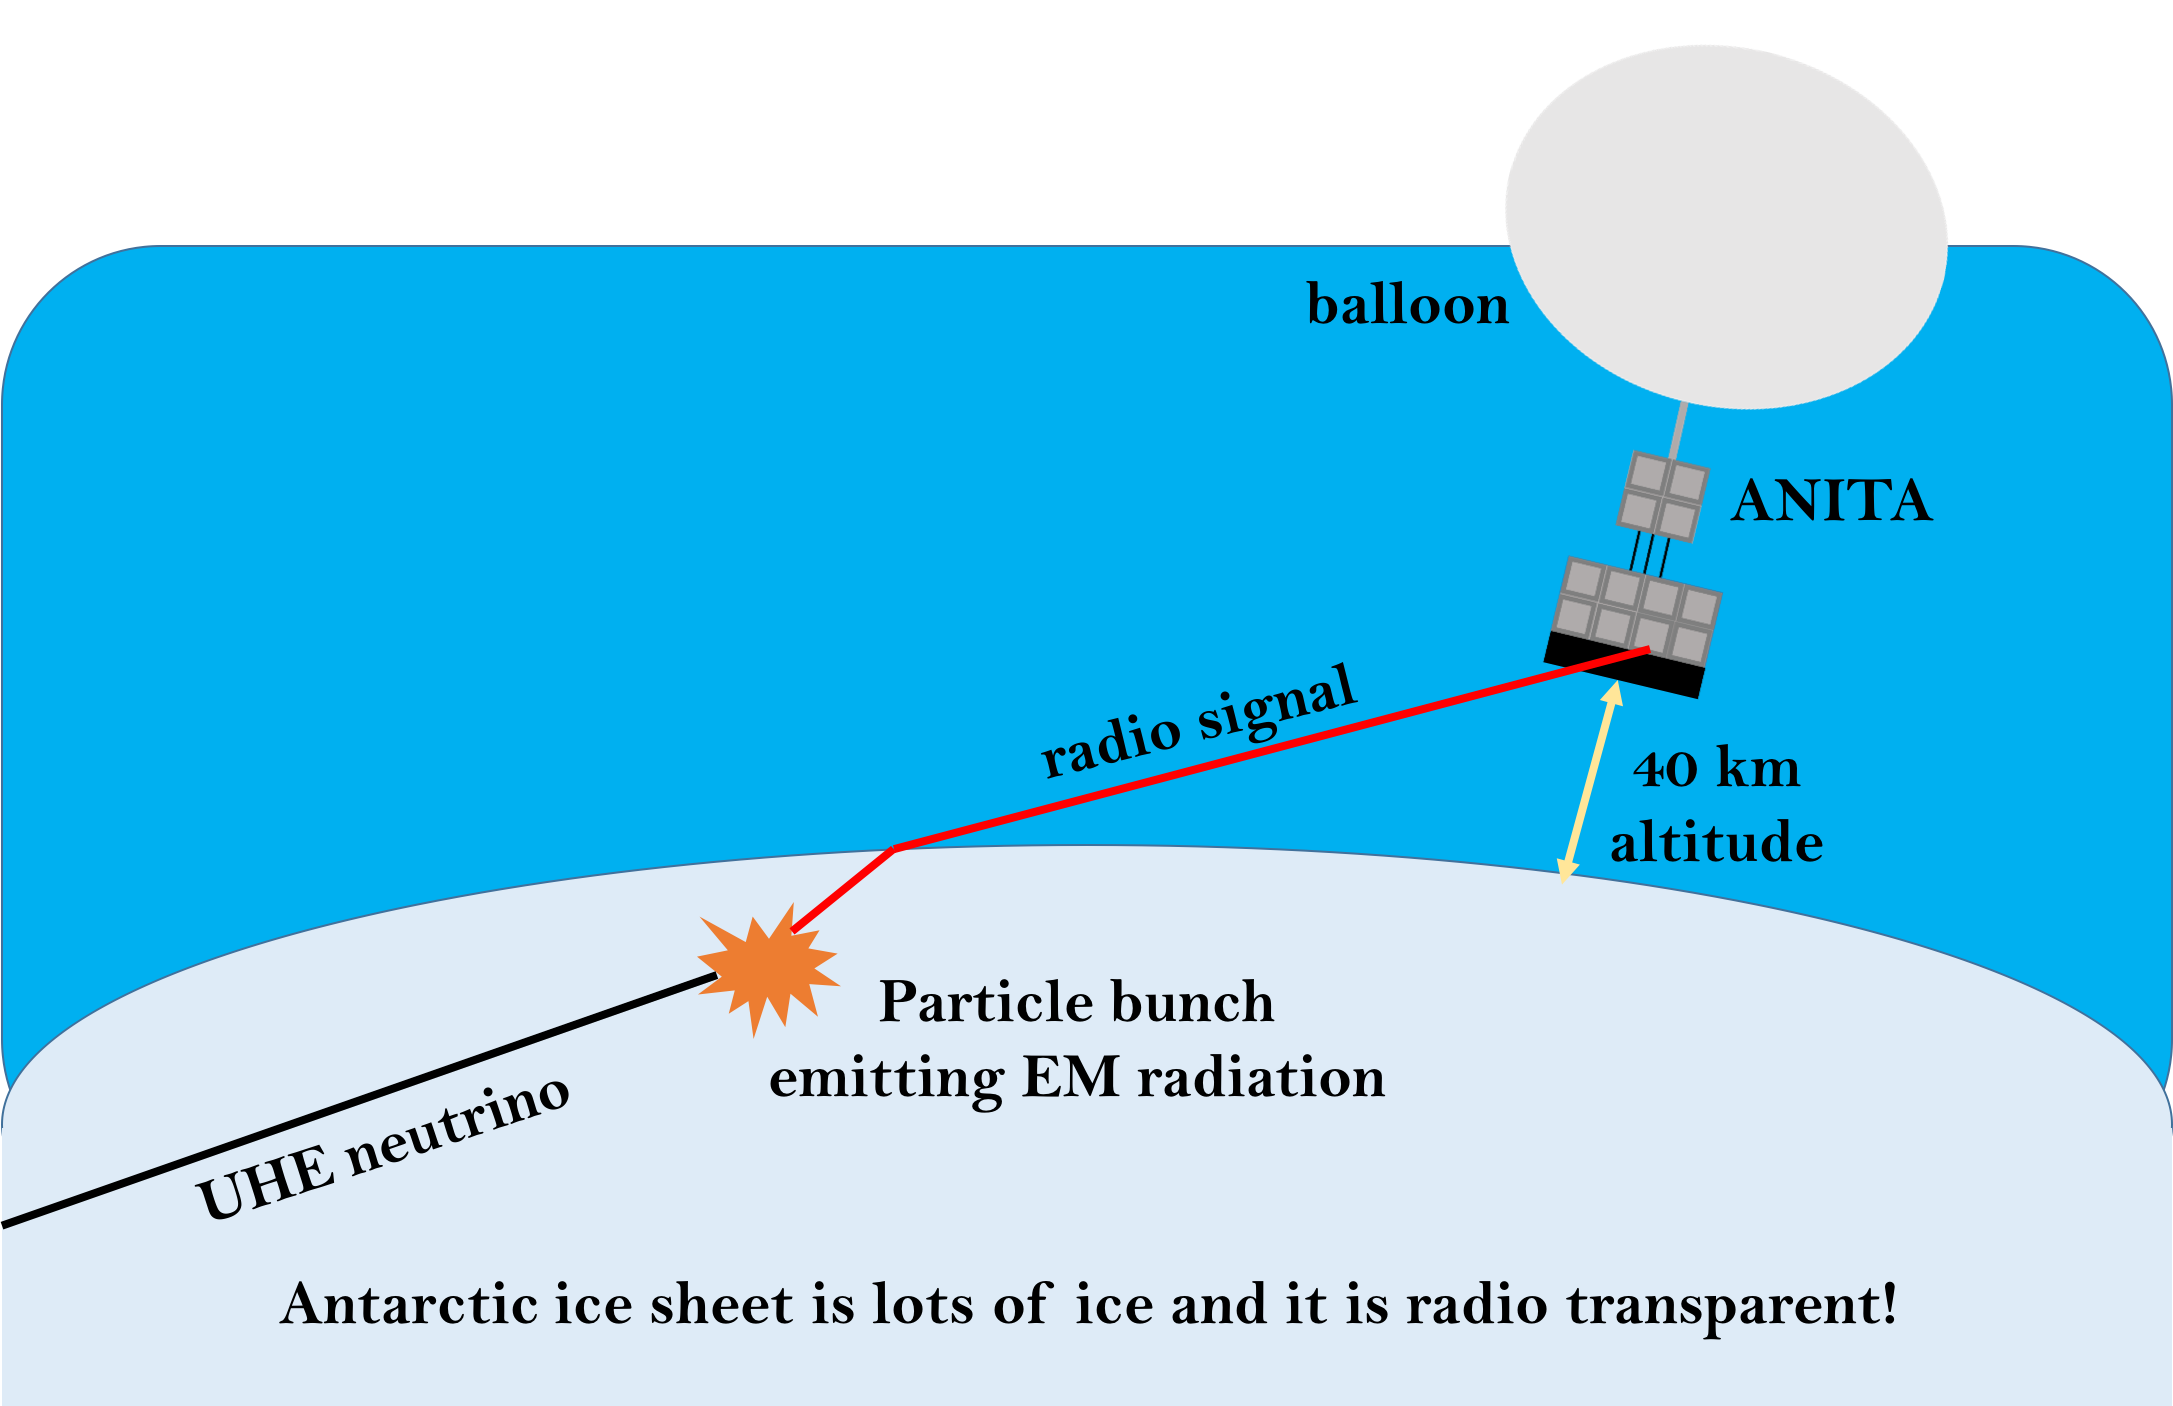
\includegraphics[width=0.9\textwidth]{figures/anita_cartoon_updated.png}
\caption{Concept of detection of UHE neutrinos with ANITA.}
\label{anita_cartoon}
\end{figure}

\subsection{ARA} 

In contrast to a balloon-borne detector such as \gls{anita}, \gls{ara} is ground-based and the \gls{ara} radio antennas are embedded in the ice of Antarctica. When ARA is deployed, it can, potentially observe all year round, as opposed to only about a month of observation time in \gls{anita}. 

The completed \gls{ara} detector will consist of 37 deep stations spaced 2~km apart at a depth of 200~m. Currently, \gls{ara} has five deep stations in the ice. A station or a single array element consists of a cluster with around 16 embedded antennas, deployed up to 200~m deep in several vertical boreholes placed with about ten meters horizontal spacing to form a small sub-array \cite{arahardware}. \gls{ara} is highly modular in that each station comprises a standalone neutrino detector for its surrounding ice. All borehole antennas have a bandwidth of 150~MHz to 1~GHz.

Like \gls{anita}, \gls{ara} too relies on the Askaryan Effect \cite{askaryan} for observation of \gls{uhe} neutrinos. ARA, too, utilizes the Antarctic ice as a target medium for neutrino interactions to look for radio signatures from these interactions. The main distinction between \gls{anita} and \gls{ara} is the area of target medium (ice) they each observe, and therefore, the neutrino energy range they are each sensitive to. \gls{anita} observes an area of roughly a million $\mathrm{km^2}$ and is sensitive to very rare neutrinos of energy $10^{18} \, \mathrm{eV}$ and above. \gls{ara} covers roughly a $200 \, \mathrm{km^2}$ area and is sensitive to the neutrino energy range of $10^{16} - 10^{19}\, \mathrm{eV}$. 

\subsection{ARA vs. IceCube} 

The main distinction between \gls{ara} and IceCube is that \gls{ara} is able to observe a hundred times bigger target volume than IceCube with fewer detector units than IceCube. This is because the attenuation length of radio signals of the frequency range that ARA detects is $\sim 1 \, \mathrm{km}$ allowing for a sparsely distributed array of detector units, whereas, the optical signals that IceCube detects are restricted to $< 100 \, \mathrm{m}$ lengths. 
The energy threshold determines the expected flux, and thus the size of the detector. 
With a smaller instrumented volume IceCube is typically sensitive to energies lower than the UHE regime, whereas, \gls{ara} is sensitive to ultra-high-energies up to $10^{19}$ eV. 


\section{Summary of remaining chapters}

The work presented in this thesis is with regard to the \gls{anita} experiment. 
Chapter~\ref{anita} describes the \gls{anita} instrument and highlights new electronics that tripled the instrument livetime of \gls{anita}. Chapter~\ref{analysis} describes the development of a new technique for analysis known as the ``binned analysis" with a focus on background reduction. The first physics results from this new analysis are presented in Chapter~\ref{results_diffuse}. Chapter~\ref{grb} is a review of \gls{grbs}, my favorite transients, in the context that these exotic events could be sources of \gls{uhe} neutrinos. Chapter~\ref{grb_technique} describes the developments in adapting the simulation and the binned analysis to a search for neutrinos from sources, specifically, \gls{grbs}. Mysteries, thoughts, ideas, and associated results are presented in Chapter~\ref{wild}.